\section{Szybka transformata Fouriera FFT dla $n=2^m$}
%%%%%%%%%%%%%%%%
\begin{frame}[allowframebreaks]{FFT}
	\begin{itemize}
		\item Danielson, Lanczos (1942)
		\item R.L.Garwin (IBM Yorktown Heights Researcg Center)
		\item James William Cooley, John Wilder Tukey (1962)
	\end{itemize}
	\begin{table}
		\centering
		\caption{Złożoność}
		\begin{tabular}{l|lll}
			& obliczeniowa && czasowa \\
			\hline
			klasyczna FT: & $O(N^2)$ & $\implies$ & 1.5 godziny \\
			FFT: & $O(N\log_2N)$ & $\implies$ & 0.1 sekundy 
		\end{tabular}
		\caption*{Założenia: \\
			rozmiar problemu: $N = 10^6$ \\
			CPU $\sim$ 100 MFLOPS}
	\end{table}
	\textbf{Dane:} $f(x_k), x_k = \frac{2\pi}{n} \cdot k, k = 0, 1, \dots, n-1$ \\
	\textbf{Szukamy:} $c_j = \frac{1}{n} \sum\limits_{k = 0}^{n-1} f(x_k) \cdot e^{-i\frac{2\pi k}{n} \cdot j}, j = 0, 1, \dots, n-1$ \\
	\textbf{gdy:} $a_k = \frac{1}{n} \cdot f(x_k), \omega = e^{-i\frac{2\pi}{n}}$ \\
	\textbf{to:} $\underline{c_j = \sum\limits_{k = 0}^{n-1} a_k \cdot \omega^{jk}}, j = 0, 1, \dots, n-1$ \\
	\textbf{Założenie:} ilość punktów: n = $2^m \implies$ tyleż współczynników Fouriera. \\
	\begin{block}{}
	(k - numer punktu) \\
	gdy k parzyste $k = 2 \cdot k_1$ \\
	gdy k nieparzyste $k = 2 \cdot k_1 + 1$ \\
	Dziedzina k: \\
	z dołu $\underline{k_1 = 0}$ (parzyste k)  \\
	z góry: $n-1 = 2^m - 1 \implies$ k - nieparzyste: $2k_1 + 1 = n-1 \implies k_1 = \frac{n}{2} - 1$ \\
	\textbf{Rozdzielamy wyznaczanie współczyników!!!: }
	\[
		c_j = \sum\limits_{k_1=0}^{\frac{n}{2} - 1} a_{2 k_1} \cdot (\omega^2)^{j \cdot k_1} + \sum\limits_{k_1 = 0}^{\frac{n}{2} - 1} a_{2  k_1 + 1} \cdot (\omega^2)^{j \cdot k_1} \cdot \omega^j
		\tag{16.24}
	\]
	\blockbreak
	\[
	\begin{cases}
		0 \leq k_1 \leq \frac{n}{2} - 1 \\
		0 \leq j \leq n-1
	\end{cases}
	\]
Dzielimy liczby $j$ na dwa zbiory wg zasady:
		\[
		j = \frac{n}{2} \cdot l + j_1 \text{ dla (reszta z dzielenia) } 0 \leq j_1 \leq \frac{n}{2} - 1
	\]
	Mniejsze od $\frac{n}{2}$
	\[
         l=0 \text{ dla }   0 \leq j \leq \frac{n}{2} - 1 
	\]
	Niemniejsze od $\frac{n}{2}$
	\[
	l=1 \text{ dla }  \frac{n}{2}  \leq j \leq n-1 
	\]
	
	\blockbreak
	z kolei:
	\[
		\underline{(\omega^2)^{jk_1}} = \omega^{2 \cdot [\frac{n}{2} \cdot l + j_1] \cdot k_1} = \omega^{n \cdot l \cdot k_1 + 2j_1k_1} = (e^{-\frac{2\pi i}{n}})^{(n \cdot l \cdot k_1 + 2j_1k_1)} = \underline{(\omega^2)^{j_1k_1}}
		\tag{bo $e^{-2\pi \cdot i  \cdot l  \cdot k_1}=1$}
	\]
	oraz
	\[
	\omega^{j} = \omega^{\frac{n}{2} \cdot l + j_1} = (e^{-\frac{2\pi i}{n}})^{\frac{n}{2}\cdot l} \cdot \omega^{j_1}=e^{-i \pi l} \cdot \omega^{j_1}
	\]
	Czyli
	\[
	\begin{cases}
		\omega^j=\omega^{j_{1}} \text{ dla } l=0 \text{ czyli }0 \leq j \leq \frac{n}{2} - 1\\
		\omega^j=-\omega^{j_{1}} \text{ dla } l=1 \text{ czyli } \frac{n}{2}  \leq j \leq n-1\\
	\end{cases}
	\]
 \blockbreak
	\underline{i uzyskujemy}:
	Dla $0 \leq j \leq \frac{n}{2} - 1$
	\[
		c_j = \underbrace{\sum\limits_{k_1 = 0}^{\frac{n}{2} - 1} a_{2 k_1} \cdot (\omega^2)^{j_1k_1}}_{\varphi(j_1)} + \underbrace{ \sum\limits_{k_1 = 0}^{\frac{n}{2}-1} a_{2 k_1+1} \cdot (\omega^2)^{j_1k_1}}_{\psi(j_1)} \cdot \omega^{j_1}, 0\leq j_1 \leq \frac{n}{2} - 1
	\]
	Dla $\frac{n}{2}  \leq j \leq n-1$
	\[
		c_j = \underbrace{\sum\limits_{k_1 = 0}^{\frac{n}{2} - 1} a_{2 k_1} \cdot (\omega^2)^{j_1k_1}}_{\varphi(j_1)} - \underbrace{ \sum\limits_{k_1 = 0}^{\frac{n}{2}-1} a_{2 k_1+1} \cdot (\omega^2)^{j_1k_1}}_{\psi(j_1)} \cdot \omega^{j_1}, 0\leq j_1 \leq \frac{n}{2} - 1
	\]
	\blockbreak
	Każdy z 2 członów jest transformatą Fouriera - zamiast pojedynczej transformaty w n punktach $\to$ suma 2 transformat w $\frac{n}{2}$ punktach wykorzystywanych dwa razy\\
Dla $0 \leq j \leq \frac{n}{2} - 1$
	\[
		c_j = \varphi(j_1) + \omega^{j_1} \cdot \psi(j_1) ; j_1 = 0, 1, \dots, \frac{n}{2} - 1
	\]
Dla $\frac{n}{2}  \leq j \leq n-1$	
	\[
		c_j = \varphi(j_1) - \omega^{j_1} \cdot \psi(j_1) ; j_1 = 0, 1, \dots, \frac{n}{2} - 1
	\]
	itd $\dots \to$ dokonując dalszych podziałów. \\
	złożoność obliczeniowa $\leq \underline{2 \cdot Nlog_2N}$ \\
	\end{block}
	\begin{center}
	\textbf{Zasada dziel i zwyciężaj!}
	\begin{figure}
	    \centering
	   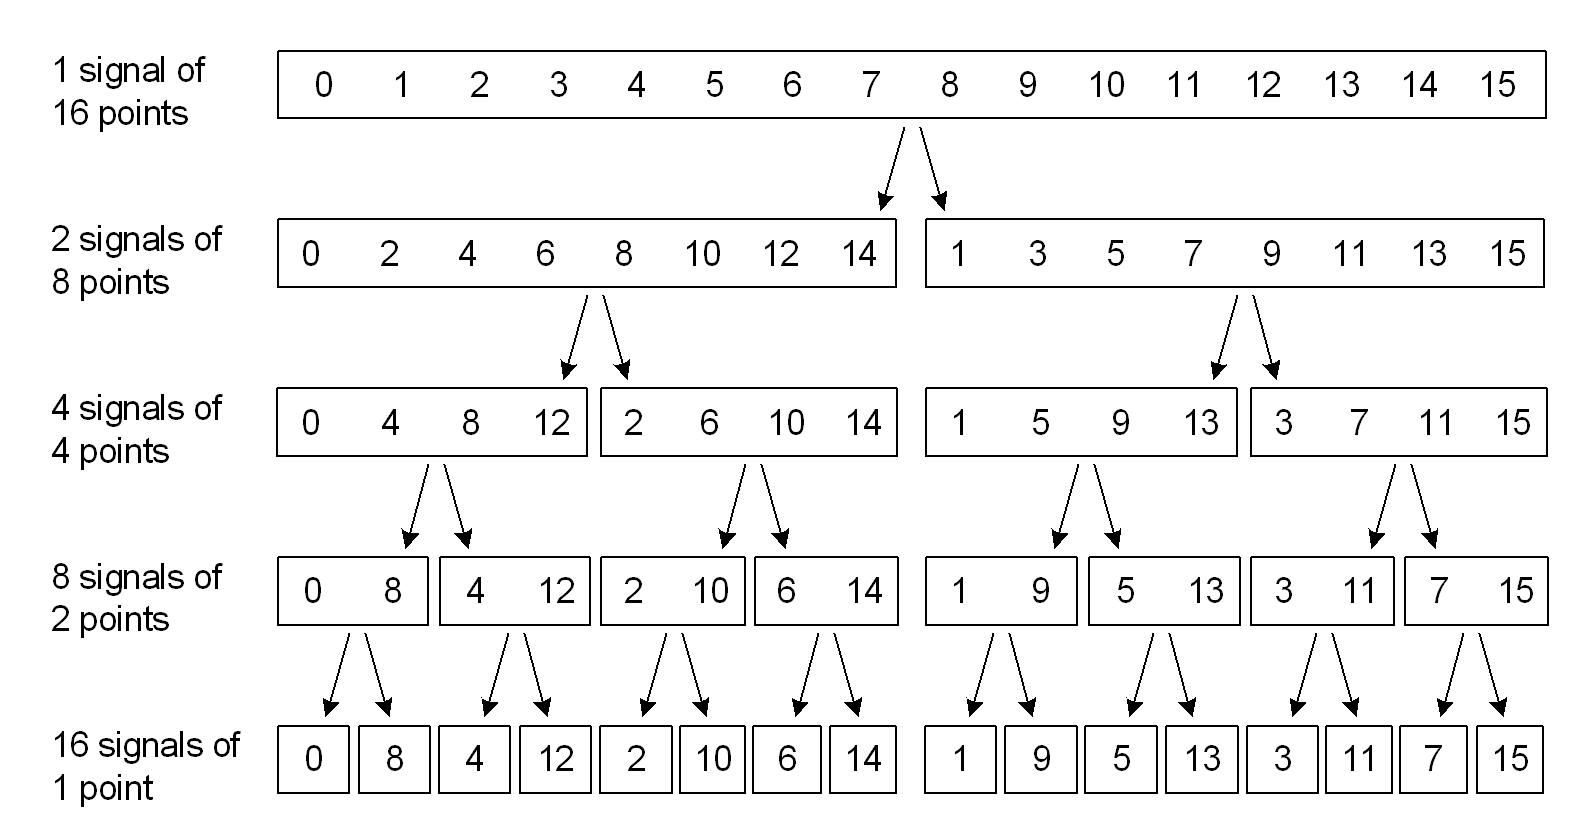
\includegraphics[width=0.8\textwidth]{img/16/podzialyFFT.png}
	    \caption{zrodlo: \url{https://riptutorial.com/algorithm/example/27088/radix-2-fft}}
	    \label{fig:my_label}
	\end{figure}
	\end{center}
	
\end{frame}  
\begin{frame}{FFT}
\begin{figure}
	    \centering
	   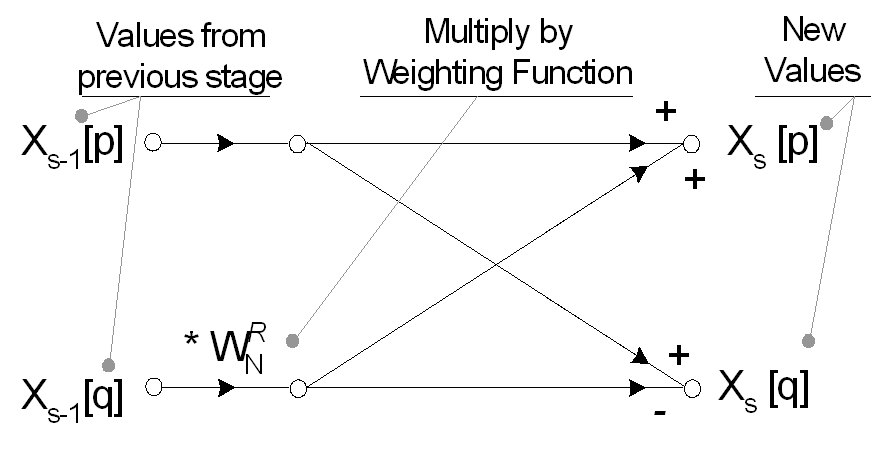
\includegraphics[width=0.9\textwidth]{img/16/bloczek_motyl.png}
	    \caption{źródlo: j.w.}
	    \label{fig:my_label}
	\end{figure}
    $W_{N}^R=(e^{\frac{-2\pi i}{N}})^R$, W naszych oznaczeniach $N=n$, $R=j_1$, $W=\omega$
\end{frame}
\begin{frame}{FFT}
    \begin{figure}
	    \centering
	   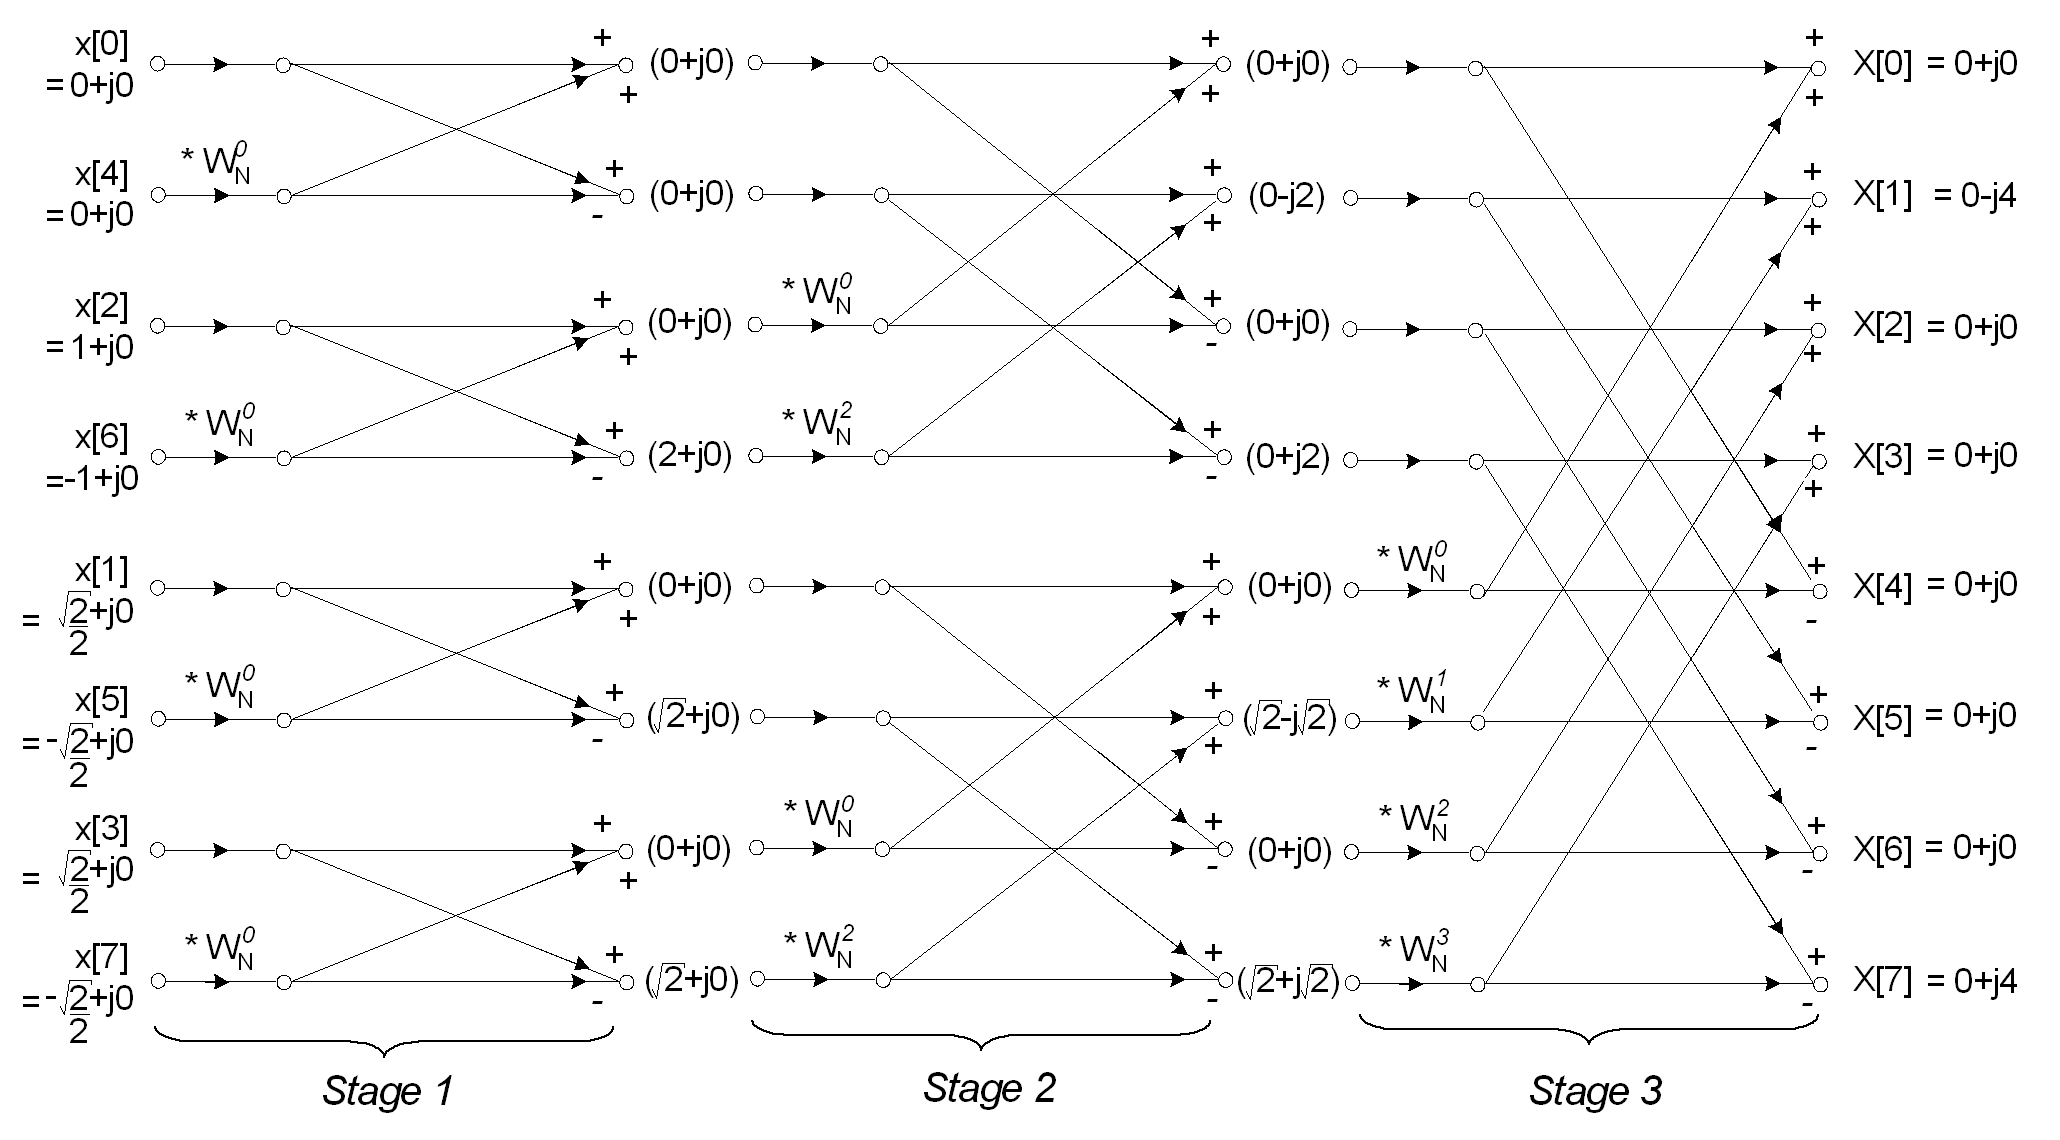
\includegraphics[width=0.8\textwidth]{img/16/motyl.png}
	    \caption{źródlo: \url{https://riptutorial.com/algorithm/example/27088/radix-2-fft}}
	    \label{fig:my_label}
	\end{figure}
\end{frame}
\begin{frame}[fragile]{Rekurencyjny algorytm FFT}
\begin{lstlisting}[language=Mathematica, mathescape]
function FFT(a)
	$n \leftarrow length[a]$
	if n = 1 
		then return a
	$\omega_n \leftarrow e^{\frac{2\pi\cdot i }{n}}$
	$\omega \leftarrow 1$
	$a_{even} \leftarrow (a_0, a_2, \dots, a_{n-2})$
	$a_{odd} \leftarrow (a_1, a_3, \dots, a_{n-1})$
	$y^{even} \leftarrow FFT(a_{even})$
	$y^{odd} \leftarrow FFT(a_{odd})$
	for j $\leftarrow$ 0 to $\frac{n}{2} -1$
		$y_j \leftarrow y^{even}_{j} + \omega y^{odd}_{j}$
		$y_{j+\frac{n}{2}} \leftarrow y^{even}_{j} - \omega y^{odd}_{j} $
		$\omega \leftarrow \omega \cdot \omega_n$
	end	
	return y
end
\end{lstlisting}

\end{frame}
\begin{frame}{Zastosowanie - szybkie mnożenie wielomianów}
\begin{itemize}
    \item Mamy dane $P(x)=\sum_{i=0}^{n-1}a_i x^i$
  oraz $Q(x)=\sum_{i=0}^{n-1}b_i x^i$
  \item Jesli potraktować $[a_i]$ oraz $[b_i]$ jak wektory, to $[c_i]$ gdzie
  $c_i=\sum_{j=0}^{i} a_j b_{i-j} $ jest ich splotem
  \item Jednocześnie:
  $W(x)=P(x)\cdot Q(x)=\sum_{i=0}^{2n-2}c_i x^i$ (aby wzór zadziałał, wyższe niż $n-1$ współczynniki $P(x)$ oraz $Q(x)$ zastępujemy 0)
  \item zamiast wyliczać współczynniki wprost: transformata $\rightarrow$ iloczyn $\rightarrow$ odwrotna transformata
\end{itemize}
\end{frame}
\begin{frame}{Splot współczynników wielomianów}
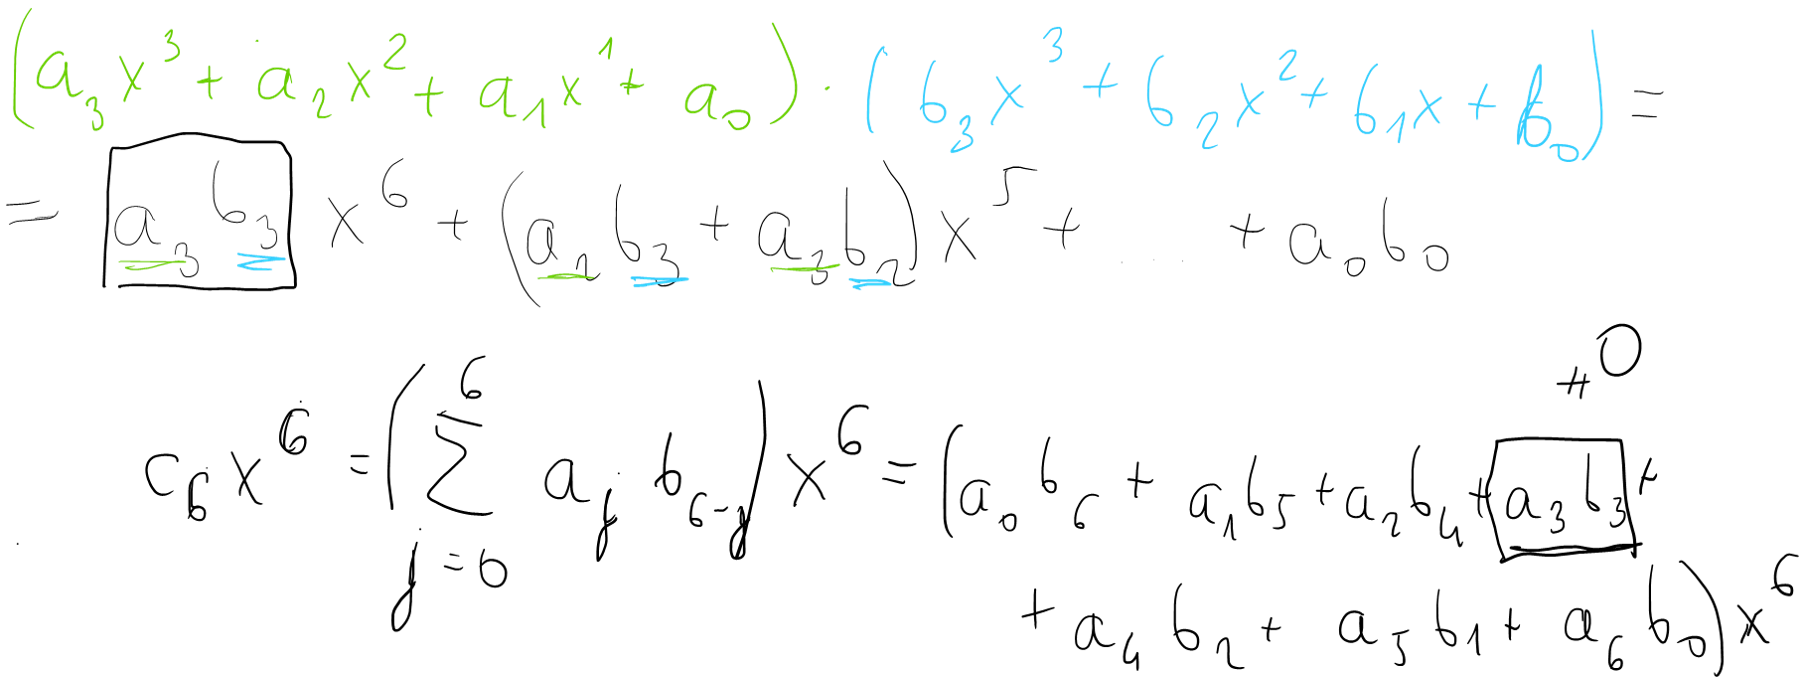
\includegraphics[width=0.99\textwidth]{img/16/splotywiel.png}    
\end{frame}
\begin{frame}{Zastosowanie - szybkie mnożenie wielomianów}
 Plan (szkic):
  \begin{enumerate}
      \item wyliczyć 2n-1 wartości wielomianów $P(x_k)$ oraz $Q(x_k)$ dla $x_k=\omega^k=e^{\frac{2\pi i k }{2n-1} }$ dla $k = 0,..,2n-2$ używając FFT (synteza) złożoność O(n log(n))
      \item policzyć wartości $W(x_k)=P(x_k)\cdot Q(x_k)$ - złożoność O(n)
      \item policzyć współczynniki $c_i$ znając wartości $W(x_k)$ - FFT (analiza) złożoność O(n log(n))
  \end{enumerate}
\end{frame}